\documentclass{beamer}
%
% Choose how your presentation looks.
%
% For more themes, color themes and font themes, see:
% http://deic.uab.es/~iblanes/beamer_gallery/index_by_theme.html
%
\mode<presentation>
{
  \usetheme{Darmstadt}      % or try Darmstadt, Madrid, Warsaw, ...
  \usecolortheme{default} % or try albatross, beaver, crane, ...
  \usefonttheme{default}  % or try serif, structurebold, ...
  \setbeamertemplate{navigation symbols}{}
  \setbeamertemplate{caption}[numbered]
} 

\usepackage[english]{babel}
\usepackage[utf8x]{inputenc}

\title[box presentation 1]{Particula Quantica En Un Pou Infinit}
\author{Cristina Raluca Vijulie, Marc Prat Masó}
\institute{Universitat Politecnica de Catalunya}
\date{\today}

\begin{document}

\begin{frame}
  \titlepage
\end{frame}

\begin{frame}{Continguts}
 \tableofcontents
\end{frame}

\section{Introducció}
\subsection{El problema: La partícula en un pou infinit}

\begin{frame}{El problema: La partícula en un pou infinit}
Tenim una partícula limitada per un alt potencial en una espai de tamany a, quines son les seves dades?
    \makebox[\textwidth][c]{
        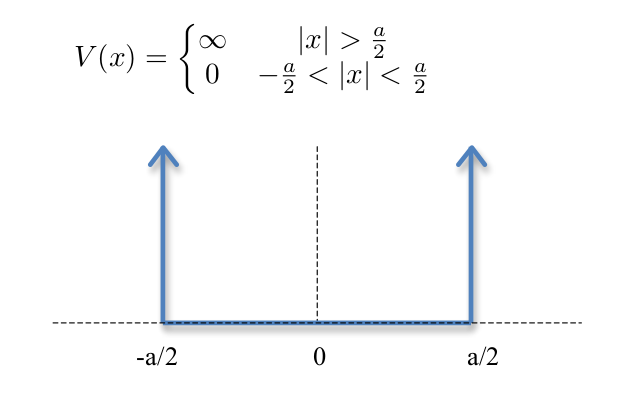
\includegraphics[width=6cm,height=4cm]{particleInBox.png}
        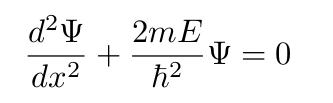
\includegraphics[width=5cm,height=2cm]{PIAB.png}

    }
\end{frame}

\subsection{El programa creat}
\begin{frame}{El programa creat}
Donats uns valors \textbf{m}, \textbf{n}, \textbf{a} el nostre programa fa:
\begin{itemize}
    \item Representar gràficament les funcions d'ona $\Psi_n$ 
    \item Dibuixar la probabilitat $|\Psi_n|^2$
    \item Representar gràficament els nivells d'energia  $E_{1..n}$
    \item Calcular la probabilitat en un punt P(x)
    \item Calcular els valors d'energia i el moment lineal $E_n $ i $ p_n$
\end{itemize}
\end{frame}

\section{Dades obtingudes}
\begin{frame}{Dades}
    \begin{itemize}
        \item Neutró
        \item Electró
        \item Protó
        \item Àtom d'hidrogen
        \item Àtom de Neó
    \end{itemize}{}
\end{frame}{}

\section{Conclusió}
\begin{frame}{Conclusió}
    \begin{itemize}
        \item $\Psi_n$: Els punts crítics van segons n i l'escala depèn de a
        \item $\Psi_n$: En n molt altes ens acostem a la física clàssica        
        \item $E_n$: Decreix molt rapit a la que no tenim un electró
        \item $p_n$: Les partícules molt pesades es moment molt lentament
    \end{itemize}{}
\end{frame}{}
\end{document}